%==============================================================================
%  Crop-Type Classification on a PASTIS Sentinel-2 Subset
%  Solafune Geo Data Scientist assignment
%
%  Build:  pdflatex report.tex   (run twice so cross-references resolve)
%  Figures are read from outputs/figures/ -- keep this file at the project root.
%==============================================================================
\documentclass[11pt,a4paper]{article}

\usepackage[T1]{fontenc}
\usepackage[utf8]{inputenc}
\usepackage{lmodern}
\usepackage[margin=2.5cm]{geometry}
\usepackage{booktabs}      % \toprule \midrule \bottomrule
\usepackage{graphicx}
\usepackage{amsmath}
\usepackage{microtype}
\usepackage{caption}
\usepackage{enumitem}
\usepackage[table]{xcolor}
\usepackage[hidelinks,colorlinks=true,linkcolor=blue!45!black,
            urlcolor=blue!45!black,citecolor=blue!45!black]{hyperref}

\graphicspath{{outputs/figures/}}

% ---- convenience macros -----------------------------------------------------
% \file{} prints a path/identifier verbatim -- underscores need no escaping,
% so you can paste raw paths straight from the repo.
\newcommand{\file}[1]{\texttt{\detokenize{#1}}}
\newcommand{\bestval}[1]{\textbf{#1}}          % highlight a winning number
% -----------------------------------------------------------------------------

\title{\textbf{Crop-Type Classification on a PASTIS Sentinel-2 Subset}}
\author{Solafune --- Geo Data Scientist Assignment}
\date{\today}

\begin{document}
\maketitle

\begin{abstract}
\noindent
The delivered model classifies crop type from a per-pixel, chronologically
ordered NDVI time series using a Random Forest, reaching \textbf{0.861
accuracy} and \textbf{0.370 macro-F1} (crop pixels only) on a spatially
disjoint test split of a
102-patch PASTIS subset. Four alternatives were evaluated under an identical
protocol. The central finding is that the \textbf{feature representation
mattered roughly three times more than the choice of model}: preserving
phenological timing improved macro-F1 by $+0.128$ with the model held fixed,
whereas swapping the model with the representation held fixed changed it by at
most $+0.038$ --- and, for neural models, changed it for the worse.
\end{abstract}

\tableofcontents
\bigskip

%==============================================================================
\section{Executive Summary}\label{sec:summary}
%==============================================================================

\textbf{Delivered model: a Random Forest on the per-pixel, chronologically
ordered NDVI time series.} Each pixel is represented by its 46 NDVI values ---
one per Sentinel-2 acquisition, in date order --- and classified into one of 18
crop/land-cover classes.

\paragraph{Evaluation protocol --- crop pixels only.}
The task is crop-type classification, so metrics are computed over the
174{,}890 test pixels whose ground truth is an actual crop (classes 1--18).
Void (19) has no ground truth, and background (0) is non-crop land cover;
neither is a crop-classification outcome, so neither is scored. Background
remains a \textbf{training} class --- the model must be able to output it, or
it would be forced to assign a crop to roads, buildings and woodland. Only the
scoring changes. Section~\ref{sec:background} reports background behaviour
separately, including the blind spot this protocol introduces.
Table~\ref{tab:headline} gives test-set performance under both protocols.

\begin{table}[htbp]
\centering
\caption{Test-set performance of the delivered model (18 held-out patches,
official PASTIS fold).}
\label{tab:headline}
\begin{tabular}{lcc}
\toprule
\textbf{Metric} & \textbf{Crop pixels only} & \textit{(background retained)} \\
\midrule
Overall accuracy                       & \bestval{0.861} & \textit{0.826} \\
Macro F1 (all 18 crop classes)         & \bestval{0.370} & \textit{0.379} \\
Macro F1 (14 classes present in test)  & \bestval{0.475} & \textit{0.481} \\
Weighted F1                            & \bestval{0.876} & \textit{0.818} \\
Mean IoU                               & \bestval{0.445} & \textit{0.418} \\
\bottomrule
\end{tabular}
\end{table}

All six crop classes holding more than 10K test pixels --- 93.9\% of the
cropped area --- score F1 between \textbf{0.89 and 0.94}.

\textbf{The central finding is that the feature representation mattered roughly
three times more than the choice of model.} Four alternatives were built and
evaluated under an identical protocol. Holding the model fixed and changing only
how the time series is represented moved macro-F1 by \textbf{$+0.128$}; swapping
the model while holding the representation fixed moved it by at most
\textbf{$+0.038$}, and in the neural case moved it \emph{backwards}.
Section~\ref{sec:why} documents this evidence, which is the justification for
the delivered model.

One caveat is carried prominently rather than buried: macro-F1 is suppressed by
the dataset, not only by the model. Four of the 18 crop classes have \textbf{zero
pixels in the test fold} and are scored 0 by construction; six more have under
2{,}000 test pixels. Section~\ref{sec:analysis} decomposes this.

%==============================================================================
\section{Introduction and Problem Statement}\label{sec:intro}
%==============================================================================

Crop-type mapping from satellite image time series supports crop monitoring,
yield estimation, and land-use analysis. Given Sentinel-2 time series and
per-pixel crop labels for a small patch subset, the task is to build a
reproducible classification pipeline, evaluate it honestly, and reason about its
limitations --- explicitly \emph{not} to chase maximum accuracy. This report
therefore prioritises a defensible representation, an evaluation protocol
without spatial leakage, and error analysis that distinguishes model failure
from dataset limitation.

%==============================================================================
\section{Dataset Description}\label{sec:dataset}
%==============================================================================

\begin{itemize}[leftmargin=*]
  \item \textbf{Source}: subset of PASTIS~\cite{garnot2021}.
  \item \textbf{102 patches}, $128 \times 128$ px at 10\,m, single Sentinel-2
        tile (\file{t31tfm}, Lambert-93 / EPSG:2154, mainland France).
  \item \textbf{10 spectral bands} (B2--B12), \textbf{46 acquisitions per
        patch}, uniformly, spanning 2018-09-20 to 2019-10-25 ($\sim$13 months).
  \item \textbf{Labels}: semantic only --- \textbf{no per-parcel instance IDs
        were provided}, so the task is pixel-level classification, not parcel
        classification. 20 class IDs (0 = Background, 1--18 = crop/land-cover,
        19 = Void/no-data).
  \item \textbf{Official 5-fold spatial CV assignment} (\file{Fold} field in
        \file{metadata.geojson}), used for the split (Section~\ref{sec:split}).
\end{itemize}

%==============================================================================
\section{Data Loading and Preparation}\label{sec:loading}
%==============================================================================

\file{src/data_loading.py} reads the \file{.npy} arrays and
\file{metadata.geojson}; \file{src/preprocessing.py} derives all features.

\begin{itemize}[leftmargin=*]
  \item \textbf{Reflectance scaling}: raw \file{int16} values are Sentinel-2 L2A
        reflectance $\times 10000$ (observed range $[-105, 14924]$; small
        negatives are normal atmospheric-correction artifacts near zero
        reflectance, not errors) --- divided by 10000 before any computation.
  \item \textbf{NDVI}:
        \[
          \mathrm{NDVI} = \frac{\mathrm{NIR} - \mathrm{Red}}{\mathrm{NIR} + \mathrm{Red}}
                        = \frac{\mathrm{B8} - \mathrm{B4}}{\mathrm{B8} + \mathrm{B4}}
        \]
        computed per acquisition, giving a $(46, 128, 128)$ cube per patch.
  \item \textbf{Sampling strategy}: the full pixel table would be $\sim$1.67M
        rows. Training instead draws up to \textbf{400 pixels per class per
        patch} (stratified, fixed seed 42), yielding 167{,}477 rows. The cap is
        a \emph{compute} device, not the class-balancing mechanism ---
        \file{class_weight='balanced'} fully equalises whatever distribution it
        receives; the cap's real contribution is geographic diversity per unit
        compute (400 pixels from each of 66 patches rather than 8{,}000 from one).
  \item \textbf{Evaluation never samples}: validation and test metrics are
        always computed over \emph{every} labelled pixel of the held-out patches
        (271{,}814 test pixels), so reported numbers reflect true full-image
        behaviour.
  \item \textbf{Void handling}: class 19 is excluded from training and from every
        reported metric --- it marks absent ground truth, not a land-cover type.
  \item \textbf{NDVI cache}: NDVI needs 2 of 10 bands, but deriving it requires
        reading the whole $(46,10,128,128)$ array ($\sim$15\,MB, $\sim$60\,MB as
        float32). \file{src/build_ndvi_cache.py} precomputes the NDVI cube once
        ($\sim$3\,MB/patch, 308\,MB total), cutting the feature-table build for
        84 patches from \textbf{995.7\,s to 1.4\,s}. All 102 patches were
        verified \textbf{bit-identical} to on-the-fly computation, so results
        are unaffected.
\end{itemize}

%==============================================================================
\section{Exploratory Data Analysis}\label{sec:eda}
%==============================================================================

Full analysis: \file{notebooks/exploration_and_training.ipynb} (executed,
outputs saved). A second notebook,
\file{notebooks/npy_profile_inspection.ipynb}, provides a per-patch raw-array
inspector.

\paragraph{Class distribution.}
Severe imbalance (Figure~\ref{fig:classdist}): Background 30.3\%, Meadow
17.8\%, Soft winter wheat 11.9\%, Corn 11.8\% --- together $\sim$72\% of
labelled pixels. Void is 8.6\%. Orchard, Beet, Potatoes, Grapevine and Winter
durum wheat are each $<$0.1\% or absent. This is why \textbf{macro-F1, not
accuracy}, is the headline metric.

\begin{figure}[htbp]
\centering
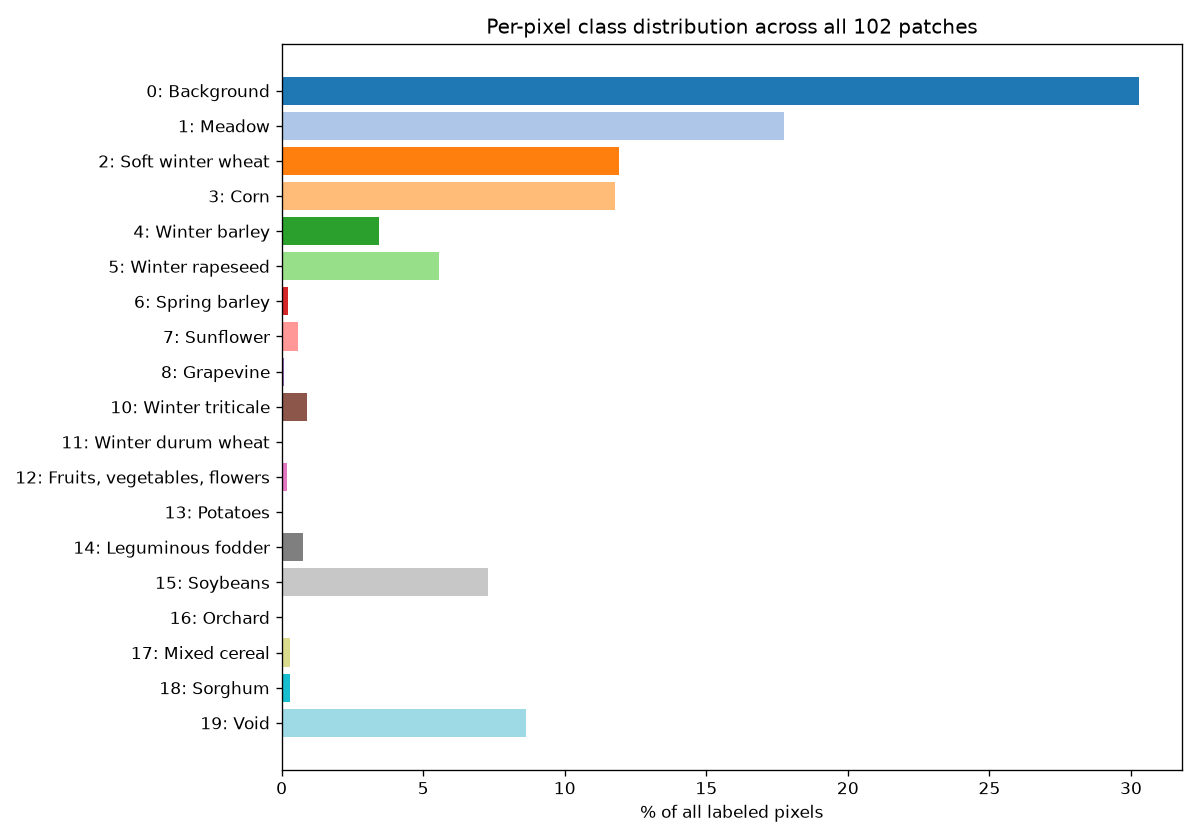
\includegraphics[width=0.85\textwidth]{class_distribution.png}
\caption{Per-pixel class distribution across all 102 patches.}
\label{fig:classdist}
\end{figure}

\paragraph{Imagery and labels.}
RGB composites (B4/B3/B2) show parcel boundaries aligning well with the label
polygons, confirming good spatial registration (Figure~\ref{fig:samples}).

\begin{figure}[htbp]
\centering
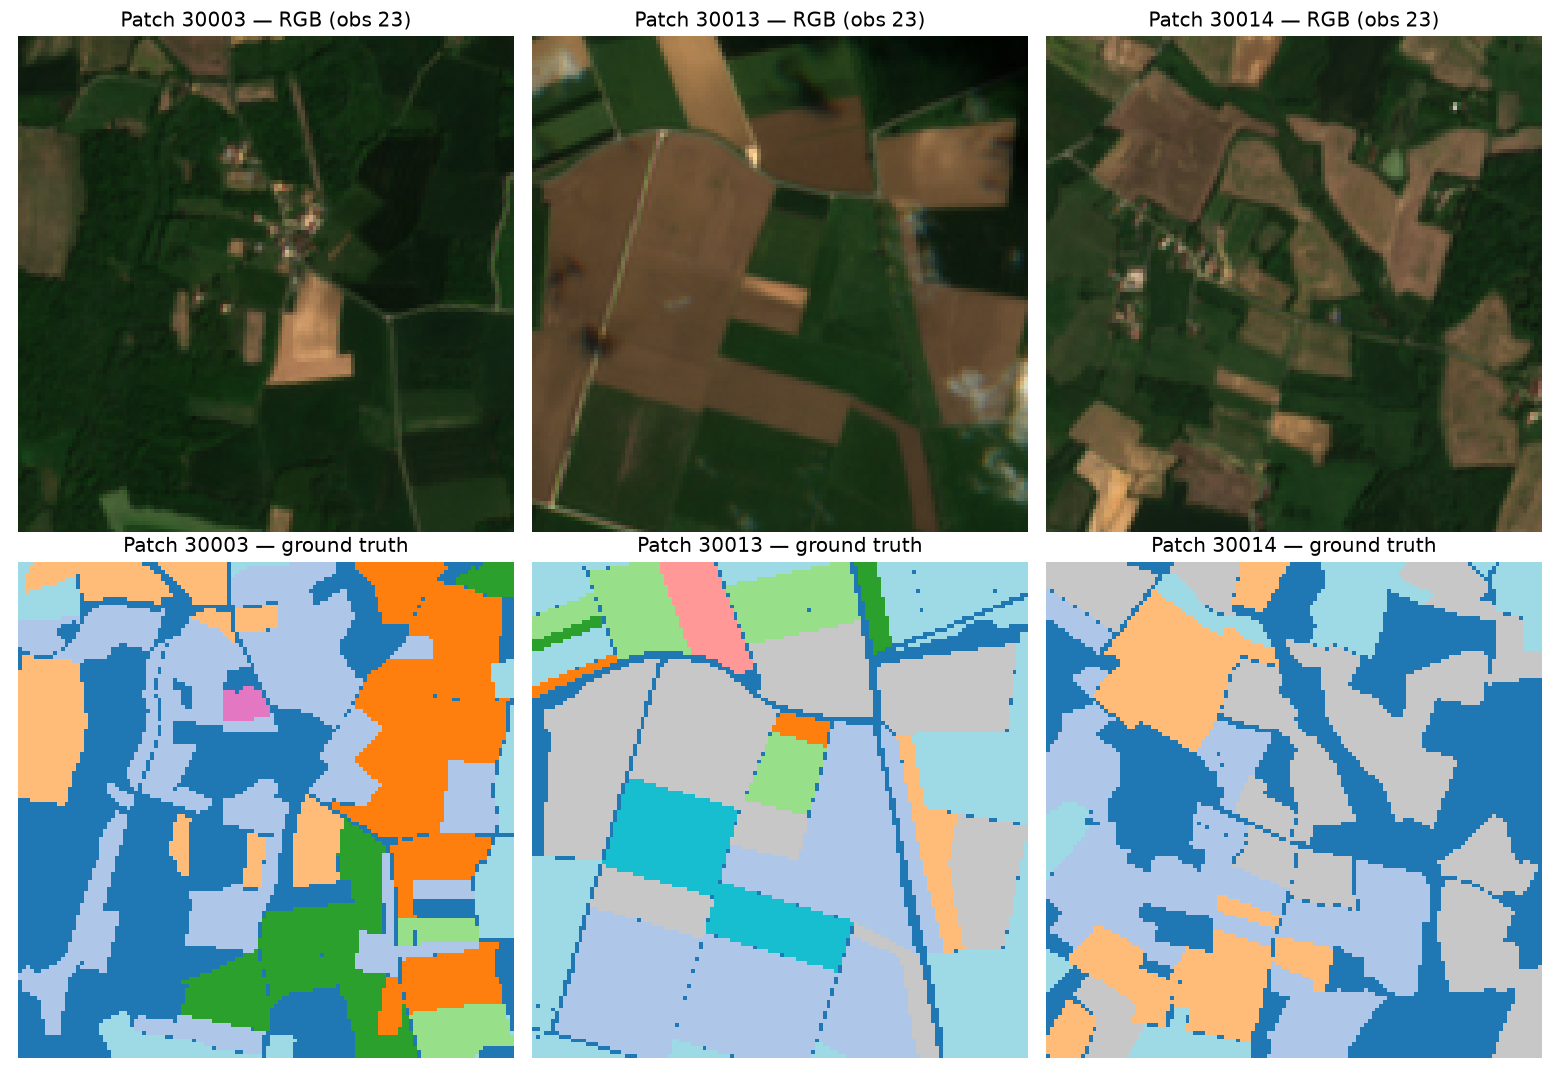
\includegraphics[width=\textwidth]{sample_patches_rgb_labels.png}
\caption{Sentinel-2 true-colour composites (top) and ground-truth label maps
(bottom) for three sample patches.}
\label{fig:samples}
\end{figure}

\paragraph{NDVI phenology --- the basis of the delivered model.}
Winter cereals green up in autumn, peak in spring, and senesce before summer;
summer row crops (corn, soybean, sunflower) stay flat through winter and peak in
July--August (Figure~\ref{fig:ndvi}). \textbf{Crop identity is encoded in
\emph{when} things happen}, not only in how green they get.

\begin{figure}[htbp]
\centering
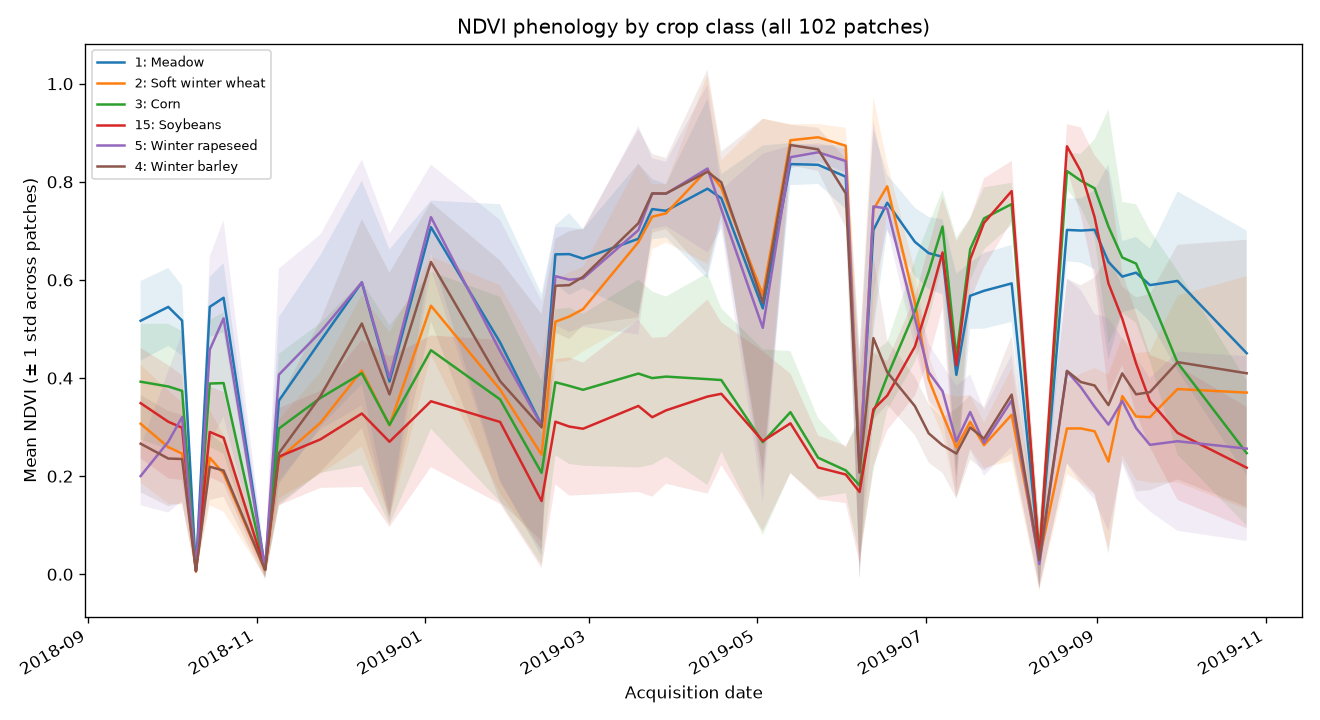
\includegraphics[width=0.9\textwidth]{ndvi_phenology_by_class.png}
\caption{Mean NDVI trajectories by crop class across all 102 patches, with
$\pm 1$ standard deviation shading. The simultaneous dips across every class on
certain dates are cloud artifacts, not phenology.}
\label{fig:ndvi}
\end{figure}

\paragraph{Area of interest.}
102 patches scattered non-contiguously across a $\sim$33 $\times$ 36\,km
bounding box within one tile (Figure~\ref{fig:aoi}), consistent with PASTIS's
spatial-diversity sampling rather than one contiguous region.

\begin{figure}[htbp]
\centering
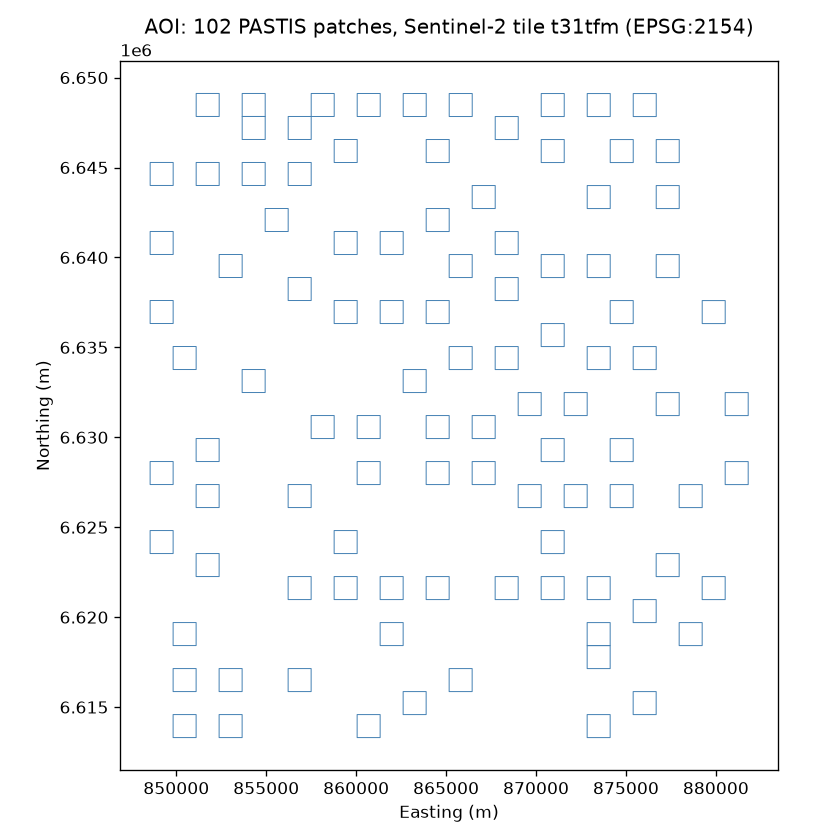
\includegraphics[width=0.6\textwidth]{aoi_extent.png}
\caption{Spatial distribution of the 102 patches in Lambert-93 (EPSG:2154).}
\label{fig:aoi}
\end{figure}

\paragraph{Data quality.}
\begin{itemize}[leftmargin=*]
  \item Sequence length is uniform (46/patch) --- no padding or masking needed,
        and all patches share one acquisition calendar (important for
        Sections~\ref{sec:method} and~\ref{sec:analysis}).
  \item Several dates show a \textbf{dataset-wide NDVI collapse across every
        class simultaneously} --- cloud/haze, not phenology. Sharpest:
        observations 3 (2018-10-10), 6 (2018-11-04) and 36 (2019-08-11), with
        mean NDVI $\approx$ 0.01--0.03 versus a typical 0.2--0.5+; milder dips at
        7, 13, 26 and 32. On individual patches this drives NDVI to physically
        impossible values (winter barley reaches $-0.55$ on 2019-08-11),
        confirming these are artifacts.
  \item Background share per patch: mean 30.3\%, max 66.7\%. Void: mean 8.6\%,
        max 29.2\%.
  \item Parcels per patch: 21--82 (median 48); on average 70.5\% of a patch lies
        inside a labelled parcel.
\end{itemize}

\subsection{Time-series decomposition, trend and change detection}\label{sec:decomposition}

\textbf{Classical seasonal-trend decomposition and change detection do not
apply to this dataset}, and saying so is more useful than producing numbers
that look meaningful (Table~\ref{tab:decomp-req}).

\begin{table}[htbp]
\centering
\caption{Why STL and BFAST are not applicable here.}
\label{tab:decomp-req}
\begin{tabular}{ll}
\toprule
\textbf{Method requirement} & \textbf{This dataset} \\
\midrule
STL: $\geq$2 full periods to separate trend from seasonal & \textbf{1.10 cycles} (400 days) \\
STL: evenly spaced samples                                & \textbf{irregular}, 5--25 day gaps \\
BFAST: multi-year series to locate land-cover change      & \textbf{one season} \\
\bottomrule
\end{tabular}
\end{table}

With 1.1 cycles the trend component is not identifiable from the seasonal term
--- they are confounded, so an STL ``trend'' would reflect the window length
rather than the crops. BFAST-family methods exist to find land-cover change
\emph{between} years; with a single season there is no such change to detect.

\paragraph{What is valid on one irregularly-sampled season}
(implemented in \file{src/phenology.py}):
\begin{enumerate}[leftmargin=*]
  \item \textbf{Harmonic (Fourier) decomposition} --- least-squares sinusoids of
        known annual period. Handles irregular sampling natively (the design
        matrix uses real acquisition dates, not sample index) and needs only one
        cycle. Splits each curve into mean level, amplitude and \textbf{phase}
        --- \emph{when} the peak occurs --- plus a residual.
  \item \textbf{Iterative outlier rejection (HANTS)} --- cloud only depresses
        NDVI, so fitting, discarding strongly negative residuals and refitting
        both reconstructs a cloud-free curve and \emph{detects} the contaminated
        dates. This is the form of change/anomaly detection that genuinely
        applies here, and it independently recovers the same cloud dates as the
        dip heuristic above.
  \item \textbf{Phenological metrics} --- SOS / POS / EOS, amplitude and
        seasonal integral (standard TIMESAT descriptors).
\end{enumerate}

\begin{table}[htbp]
\centering
\caption{Crop calendar recovered from the data alone, with no agronomic input
(\file{outputs/metrics/phenology_metrics.csv}).}
\label{tab:phenology}
\begin{tabular}{lccccr}
\toprule
\textbf{Class} & \textbf{Amplitude} & \textbf{SOS} & \textbf{Peak} & \textbf{EOS} & \textbf{Season (d)} \\
\midrule
Winter barley     & 0.250 & 2019-02-01 & \textbf{2019-04-13} & 2019-06-09 & 128 \\
Winter rapeseed   & 0.209 & 2019-01-30 & \textbf{2019-05-03} & 2019-06-24 & 145 \\
Soft winter wheat & 0.283 & 2019-02-20 & \textbf{2019-05-03} & 2019-06-27 & 127 \\
Winter triticale  & 0.240 & 2019-02-21 & \textbf{2019-05-03} & 2019-06-24 & 123 \\
Meadow            & 0.140 & 2019-02-13 & 2019-05-03          & 2019-08-22 & 189 \\
Spring barley     & 0.189 & 2019-04-03 & \textbf{2019-06-02} & 2019-08-04 & 123 \\
Sunflower         & 0.179 & 2019-05-24 & \textbf{2019-07-17} & 2019-09-08 & 106 \\
Soybeans          & 0.167 & 2019-06-13 & \textbf{2019-08-11} & 2019-09-28 & 107 \\
Corn              & 0.144 & 2019-06-21 & \textbf{2019-08-11} & 2019-10-01 & 103 \\
\bottomrule
\end{tabular}
\end{table}

\begin{figure}[htbp]
\centering
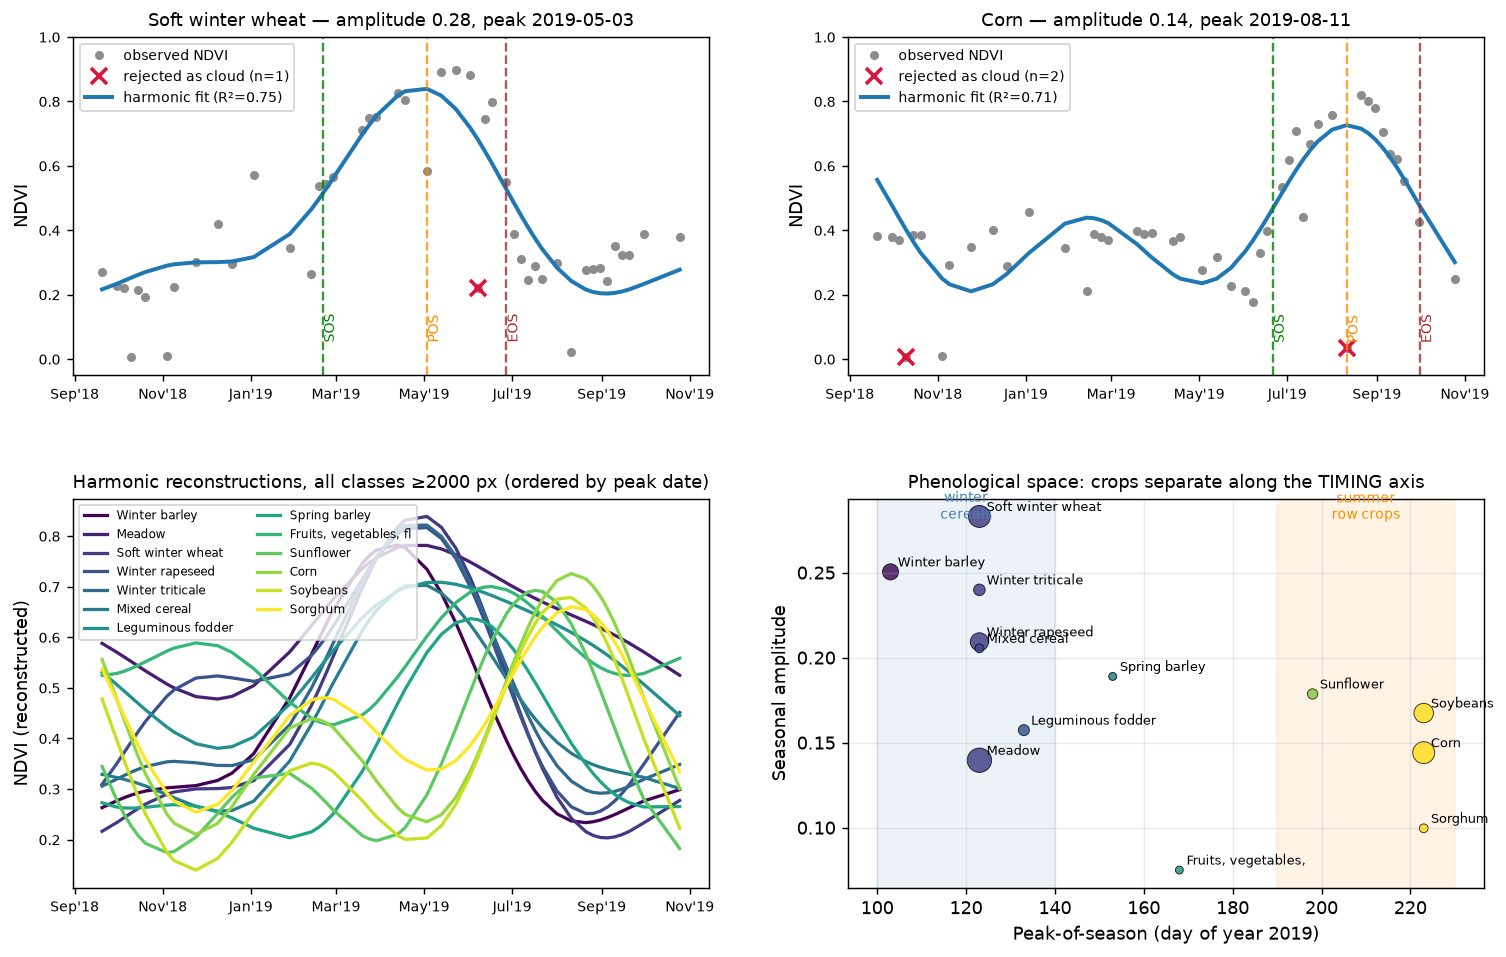
\includegraphics[width=\textwidth]{phenology_decomposition.png}
\caption{Top: harmonic decomposition of two contrasting crops, with
cloud-rejected acquisitions marked ($\times$) and SOS/POS/EOS annotated.
Bottom left: reconstructed seasonal curves for all classes with $\geq$2000 px,
ordered by peak date. Bottom right: phenological space --- classes separate
along the \emph{timing} axis far more cleanly than along amplitude.}
\label{fig:phenology}
\end{figure}

The peak-of-season ordering in Table~\ref{tab:phenology} is a textbook crop
calendar obtained with no agronomic input: winter barley (13 Apr)
$\rightarrow$ winter cereals and rapeseed (3 May) $\rightarrow$ spring barley
(2 Jun) $\rightarrow$ sunflower (17 Jul) $\rightarrow$ corn and soybean
(11 Aug) --- a \textbf{120-day spread in peak date}.

\textbf{This is the quantitative basis for the delivered model.} In the
amplitude-versus-peak-date plane (Figure~\ref{fig:phenology}, bottom right),
classes separate far better \emph{horizontally} (timing) than
\emph{vertically}: amplitude spans a narrow 0.08--0.28 and overlaps heavily
between the winter and summer groups, while peak date splits them into two
clusters four months apart. A representation preserving \emph{when} can exploit
that axis; order-invariant statistics cannot see it at all ---
Section~\ref{sec:why} measures the cost at \textbf{$+0.128$ macro-F1}.

Two caveats stated rather than buried:
\begin{itemize}[leftmargin=*]
  \item $R^2$ is computed on \textbf{retained} points, so it measures fit on the
        cloud-screened series. Aggressive rejection inflates it: at
        \file{reject_sigma=1.5} some classes lost more than 50\% of their
        observations and reported $R^2>0.97$ on the survivors. The default of
        2.5 is where recovered amplitude and peak date stabilise, with a hard
        25\% cap on rejection.
  \item Low-amplitude, poorly-fit classes (Sorghum: amplitude 0.10,
        $R^2=0.42$) have unreliable SOS/EOS --- too flat for a threshold
        crossing to be well defined. Peak date remains meaningful; season length
        does not.
\end{itemize}

%==============================================================================
\section{Train / Validation / Test Split}\label{sec:split}
%==============================================================================

The split is summarised in Table~\ref{tab:split}.

\begin{table}[htbp]
\centering
\caption{Split by official PASTIS fold.}
\label{tab:split}
\begin{tabular}{lcc}
\toprule
\textbf{Split} & \textbf{Folds} & \textbf{Patches} \\
\midrule
Train      & 1, 2, 3 & 66 \\
Validation & 4       & 18 \\
Test       & 5       & 18 \\
\bottomrule
\end{tabular}
\end{table}

The \textbf{official PASTIS fold assignment} is used rather than a random
shuffle. PASTIS's folds are spatially disjoint; a random per-patch split risks
spatial autocorrelation leakage, where neighbouring patches sharing soil,
weather and farm management land on both sides of the split and inflate
reported performance. Patch IDs are written to
\file{configs/splits/train.txt}, \file{val.txt} and \file{test.txt} by
\file{src/make_splits.py}, so the split is exactly reproducible. This choice
makes the numbers \emph{lower} and more honest --- that is its purpose.

%==============================================================================
\section{Methodology --- The Delivered Model}\label{sec:method}
%==============================================================================

\textbf{Representation} (\file{src/preprocessing.py}, function
\file{patch_ndvi_series}): each pixel is a 46-dimensional vector
\file{ndvi_t00} \ldots \file{ndvi_t45}, the NDVI at each acquisition in
chronological order. No summary statistics, no other bands.

The rationale is direct: a tree splitting on \file{ndvi_t28 > 0.6} asserts
``still green in mid-June,'' exactly the phenological statement that separates
autumn-sown cereals from summer row crops (Section~\ref{sec:eda}). Preserving
order preserves that information.

\textbf{Model}: Random Forest --- 300 trees, \file{max_depth=20},
\file{class_weight='balanced'}, seed 42 (\file{configs/config.yaml}, section
\file{model_ndvi}).

\textbf{Class imbalance}: \file{class_weight='balanced'} (inverse-frequency),
plus the stratified sampling of Section~\ref{sec:loading}.

\textbf{Compute}: CPU only. Feature build 1.4\,s with the NDVI cache (29\,s
cold), Random Forest fit 138\,s. The complete pipeline reproduces in
\textbf{under three minutes} on a laptop with no GPU, via
\file{python build_ndvi_cache.py} followed by \file{python train.py --track ndvi}.

%==============================================================================
\section{Why This Representation --- Supporting Evidence}\label{sec:why}
%==============================================================================

The delivered model was chosen on evidence, not preference. Three alternatives
were built and evaluated under the \emph{identical} split, sampling, void
handling and metric code, so differences are attributable to the design change
alone (Table~\ref{tab:alternatives}). Table~\ref{tab:ablation} then isolates
each design variable in turn.

\begin{table}[htbp]
\centering
\caption{All evaluated models, identical protocol. Track C is delivered.}
\label{tab:alternatives}
\begin{tabular}{llccc}
\toprule
\textbf{Track} & \textbf{Representation} & \textbf{Model} & \textbf{Accuracy} & \textbf{Macro F1} \\
\midrule
\textbf{C (delivered)} & 46 ordered NDVI values & Random Forest & \bestval{0.861} & \bestval{0.370} \\
D & 46 ordered NDVI values & TempCNN (249K params)     & 0.824 & 0.360 \\
A & 60 temporal statistics & XGBoost                   & 0.726 & 0.280 \\
A & 60 temporal statistics & Random Forest             & 0.654 & 0.242 \\
B & raw $(T,C,H,W)$, 10 bands & Temporal-Attn U-Net (491K, 40 ep) & 0.712 & 0.340 \\
\bottomrule
\end{tabular}
\end{table}

\begin{table}[htbp]
\centering
\caption{Isolating each design variable.}
\label{tab:ablation}
\begin{tabular}{llc}
\toprule
\textbf{Comparison} & \textbf{Held fixed} & \textbf{$\Delta$ Macro F1} \\
\midrule
temporal stats $\rightarrow$ ordered NDVI & model = Random Forest      & \bestval{$+0.128$} \\
Random Forest $\rightarrow$ XGBoost       & features = temporal stats  & $+0.038$ \\
Random Forest $\rightarrow$ TempCNN       & features = ordered NDVI    & $-0.009$ \\
\bottomrule
\end{tabular}
\end{table}

\paragraph{Why the statistics representation fails.}
Track~A described each band by its temporal mean, standard deviation, minimum,
maximum and slope. Four of those five are \textbf{permutation-invariant in
time} --- shuffling the 46 acquisitions leaves them bit-identical (verified
directly; only \file{slope} changes). That representation encodes \emph{how
much} vegetation there was and almost nothing about \emph{when}. Given that crop
identity is a timing signal, this is a fundamental mismatch, and it costs 0.128
macro-F1. Switching to the ordered series improved \textbf{every one of the 14
crop classes present in the test set} (mean $+0.164$, no class made worse), led
by Sunflower ($0.141 \rightarrow 0.802$) and Winter barley
($0.383 \rightarrow 0.920$).

\paragraph{Why the neural models did not win.}
Both networks underperformed the Random Forest, for a statistical rather than an
architectural reason: \textbf{the effective sample size is 66 patches, not
167{,}477 pixels}. Pixels within a parcel share soil, weather and one farmer's
decisions --- they are near-duplicates, not independent observations. Fitting
249K--491K parameters against $\sim$66 independent units overfits, whereas a
Random Forest's bagging and feature subsampling are robust in exactly that
regime. The evidence is visible in training: the TempCNN drove training loss
from 0.87 to 0.10 while validation macro-F1 plateaued at $\sim$0.42 from epoch
15 onward.

The U-Net was additionally trained to full convergence (40 epochs, $\sim$1.9\,h
CPU) to ensure it was not dismissed on an under-trained result. It improved from
0.293 to 0.332 macro-F1 --- real, but insufficient, and still 0.228 behind on
accuracy. Its validation macro-F1 oscillated between 0.219 and 0.400
($\sigma = 0.047$) across the final 20 epochs, so its best-checkpoint value of
0.400 is substantially selection-on-noise; test came in at 0.332. The delivered
model shows no comparable instability.

%==============================================================================
\section{Results}\label{sec:results}
%==============================================================================

\subsection{Per-class performance (test set)}\label{sec:perclass}

Table~\ref{tab:perclass} gives per-class precision, recall and F1;
Figure~\ref{fig:cm} shows the corresponding row-normalised confusion matrix.

\begin{table}[htbp]
\centering
\caption{Per-class test metrics for the delivered model.}
\label{tab:perclass}
\begin{tabular}{lrccc}
\toprule
\textbf{Class} & \textbf{Support (px)} & \textbf{Precision} & \textbf{Recall} & \textbf{F1} \\
\midrule
Meadow                    & 54{,}359 & 0.939 & 0.853 & 0.894 \\
Soft winter wheat         & 35{,}388 & 0.921 & 0.934 & 0.928 \\
Corn                      & 31{,}525 & 0.917 & 0.931 & 0.924 \\
Winter rapeseed           & 17{,}328 & 0.948 & 0.924 & 0.936 \\
Soybeans                  & 13{,}828 & 0.913 & 0.924 & 0.919 \\
Winter barley             & 11{,}780 & 0.939 & 0.901 & 0.920 \\
Sunflower                 &  2{,}851 & 0.943 & 0.698 & 0.802 \\
Fruits/vegetables/flowers &  2{,}643 & 0.000 & 0.000 & 0.000 \\
Leguminous fodder         &  1{,}778 & 0.653 & 0.182 & 0.285 \\
Winter triticale          &  1{,}612 & 0.067 & 0.035 & 0.046 \\
Mixed cereal              &      674 & 0.000 & 0.000 & 0.000 \\
Sorghum                   &      665 & 0.000 & 0.000 & 0.000 \\
Winter durum wheat        &      306 & 0.000 & 0.000 & 0.000 \\
Spring barley             &      153 & 0.000 & 0.000 & 0.000 \\
\midrule
Beet, Grapevine, Potatoes, Orchard & 0 & --- & --- & --- \\
\bottomrule
\end{tabular}
\end{table}

\begin{figure}[htbp]
\centering
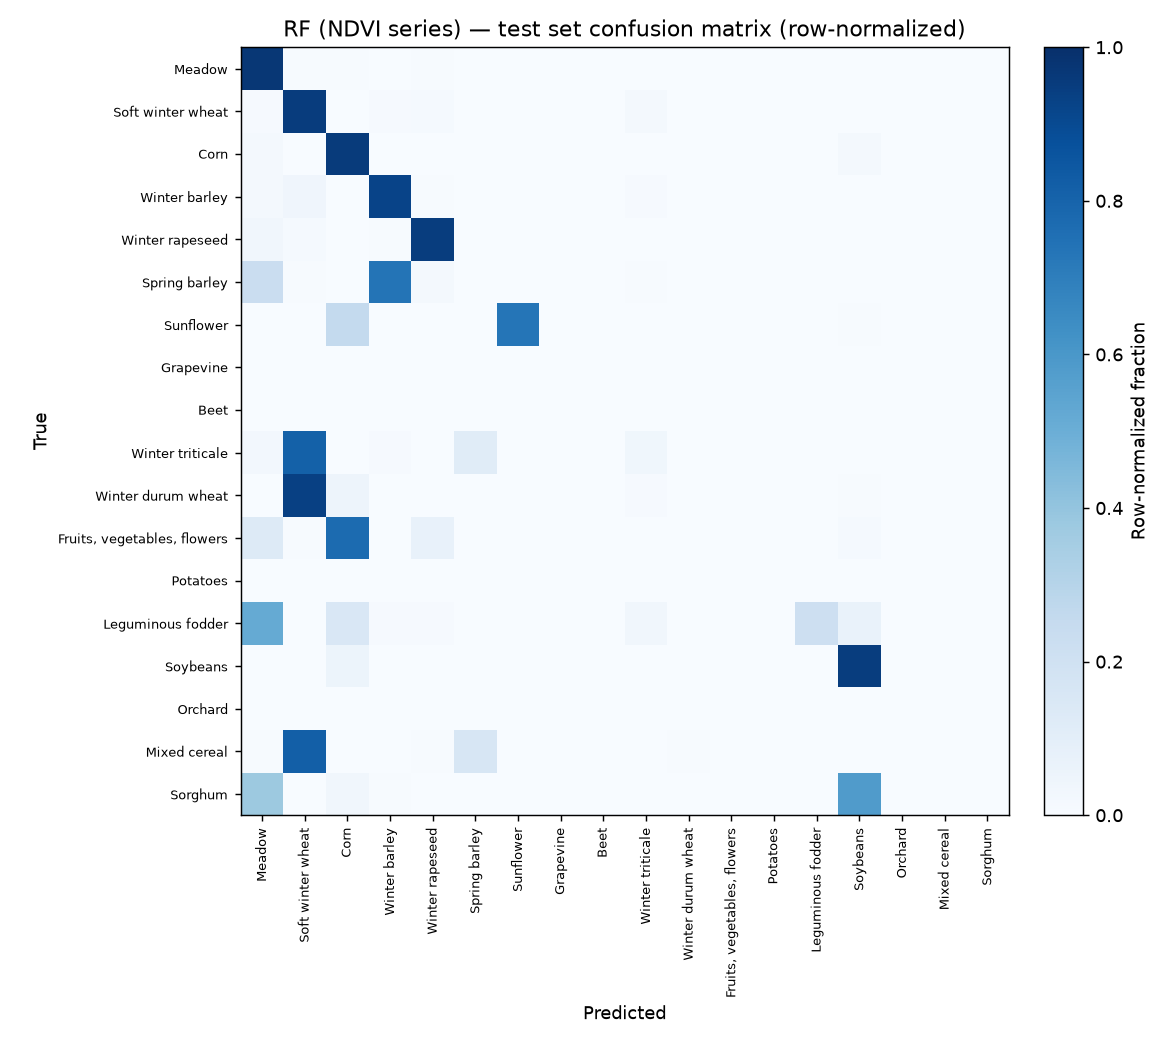
\includegraphics[width=0.62\textwidth]{confusion_matrix_ndvi_rf_test.png}
\caption{Row-normalised test-set confusion matrix for the delivered model.}
\label{fig:cm}
\end{figure}

\subsection{The model recovered the crop calendar}\label{sec:calendar}

Because every feature \emph{is} a date, the Random Forest's feature importances
read out directly as phenology
(\file{outputs/metrics/ndvi_rf_feature_importance.csv}). The five most
informative acquisitions are 2019-06-17 (0.049), 2019-06-02 (0.048), 2019-05-23
(0.038), 2019-08-21 (0.035) and 2019-05-13 (0.033).

\textbf{Ten dates in the April--June window carry 30.5\% of total importance}
--- the period when winter cereals senesce while summer row crops are greening
up, i.e.\ precisely when the two groups are maximally separable. The model
independently rediscovered the agronomic discrimination window visible in
Figure~\ref{fig:ndvi}, which is meaningful evidence it learned real phenology
rather than an artifact. This interpretability is a practical argument for the
representation independent of its accuracy.

\subsection{Background --- the afterthought, quantified}\label{sec:background}

Background is excluded from the headline metrics because it is not a crop. That
exclusion is deliberate but not free, and this section states its cost rather
than leaving it implicit (Table~\ref{tab:background}).

\begin{table}[htbp]
\centering
\caption{Background interactions for the delivered model on the test set.}
\label{tab:background}
\begin{tabular}{lrc}
\toprule
\textbf{Direction} & \textbf{Count} & \textbf{Scored?} \\
\midrule
Crop pixels predicted as background & 11{,}701 / 174{,}890 (\textbf{6.7\%}) & Yes --- a recall miss \\
Background pixels predicted as a crop & 23{,}024 / 96{,}924 (\textbf{23.8\%}) & \textbf{No} --- invisible \\
\bottomrule
\end{tabular}
\end{table}

The second row is the blind spot. Roughly a quarter of background pixels are
assigned some crop label, and \textbf{79\% of those errors land on Meadow}
(18{,}233\,px), the remainder spread over Corn (1{,}570), Soft winter wheat
(1{,}078), Winter barley (893) and Winter rapeseed (622).

The consequence is visible in the precision column: excluding background-truth
pixels removes those false positives from the denominator, so crop precision
rises --- Meadow from \textbf{0.686 to 0.939}, Winter barley 0.870 to 0.939,
Corn 0.874 to 0.917. Meadow is the extreme case because it is spectrally and
phenologically closest to unmanaged grassy background.

\paragraph{How to read this.}
For the assignment's question --- \emph{given a crop pixel, is the crop
identified correctly?} --- the crop-only numbers are the right ones. For an
operational crop-mapping product running over whole scenes including
non-agricultural land, the with-background numbers (\file{*_withbg_*}) are the
honest ones, because commission onto background is a real map error. Both are
reported for exactly this reason. A parcel mask, or the parcel polygons already
present in \file{metadata.geojson}, would remove most of this error class in
deployment.

%==============================================================================
\section{Analysis and Interpretation}\label{sec:analysis}
%==============================================================================

\subsection{Macro-F1 is suppressed by the dataset, not only the model}

Reading 0.370 as ``the model is 37\% good'' would be wrong
(Table~\ref{tab:buckets}).

\begin{table}[htbp]
\centering
\caption{Decomposition of macro-F1 by class support.}
\label{tab:buckets}
\begin{tabular}{lrrc}
\toprule
\textbf{Bucket} & \textbf{Classes} & \textbf{Share of test px} & \textbf{Mean F1} \\
\midrule
$>$10K px   & 6 & \bestval{93.9\%} & \bestval{0.920} \\
2K--10K px  & 2 & 3.1\%            & 0.401 \\
$<$2K px    & 6 & 3.0\%            & 0.055 \\
\textbf{0 px} & \textbf{4} & \textbf{0\%} & \textbf{0.000 (forced)} \\
\bottomrule
\end{tabular}
\end{table}

\file{Grapevine}, \file{Beet}, \file{Potatoes} and \file{Orchard} have \textbf{no
pixels in the test fold} --- Beet appears nowhere in the subset at all, and the
other three occur in exactly one training patch each. They cannot be scored, yet
they enter the macro average as four hard zeros. Excluding them raises macro-F1
from 0.370 to \textbf{0.475}. Both numbers are reported throughout rather than
silently choosing the flattering one.

The top row is the practical headline: on the six crop classes making up 94\%
of the cropped area, mean F1 is \textbf{0.920}.

\subsection{Rare-class failure is about patches, not pixels}

Test F1 tracks the number of training \emph{patches} far more closely than the
number of training pixels (Table~\ref{tab:patches}).

\begin{table}[htbp]
\centering
\caption{Test F1 tracks the number of training \emph{patches}, not pixels.}
\label{tab:patches}
\begin{tabular}{lrrc}
\toprule
\textbf{Class} & \textbf{Train patches} & \textbf{Train px} & \textbf{Test F1} \\
\midrule
Meadow / Corn / Soft winter wheat  & 60--65 & 115K--198K & 0.89--0.93 \\
Winter barley                      & 42     & 34{,}871   & 0.920 \\
Winter rapeseed                    & 38     & 56{,}030   & 0.936 \\
Winter triticale                   & 18     & 10{,}335   & 0.046 \\
Sunflower                          & 8      & 4{,}607    & 0.802 \\
Fruits/vegetables/flowers          & 3      & 500        & 0.000 \\
Grapevine, Durum wheat, Potatoes, Orchard & \textbf{1} & 75--1{,}345 & n/a \\
\bottomrule
\end{tabular}
\end{table}

Every class in $\geq$38 training patches scores $>$0.89; classes appearing in
$\leq$3 patches fail entirely. Three patches of ``Fruits/vegetables/flowers'' is
effectively $n = 3$ regardless of pixel count --- the same
patch-level-independence argument that explains the neural models' overfitting
(Section~\ref{sec:why}).

\subsection{Confusions are agronomically coherent}

Errors are systematic, not random: each failing class collapses into its nearest
agronomic relative.

\begin{itemize}[leftmargin=*]
  \item \textbf{Winter triticale $\rightarrow$ 75\% Soft winter wheat.}
        Triticale is a wheat$\times$rye hybrid with a nearly identical calendar;
        wheat has $\sim$11$\times$ more training pixels, so the classifier has
        every incentive to absorb it. Notably this class did \emph{not} improve
        when timing was restored --- its failure is genuine spectral-temporal
        near-identity plus imbalance, not representation.
  \item \textbf{Sorghum $\rightarrow$ 81\% Corn} (both summer C4 row crops).
  \item \textbf{Spring barley $\rightarrow$ Winter barley + wheat} (same genus).
  \item \textbf{Mixed cereal $\rightarrow$ scattered} across soybean, barley and
        wheat --- by definition a mixture with no single signature.
\end{itemize}

That the errors are interpretable is evidence the features carry real signal:
the model fails where the underlying classes are genuinely close, not at random.

\subsection{Effects of resolution, cloud, and timing}

At 10\,m, pixels near parcel boundaries mix multiple crops, producing the
residual salt-and-pepper noise visible in Section~\ref{sec:viz} --- the main
cost of per-pixel classification without spatial smoothing. The
cloud-contaminated dates identified in Section~\ref{sec:eda} inject noise
directly into the feature vector: for this model a clouded acquisition corrupts
one feature outright rather than being diluted across a temporal average. That
performance remains high suggests the Random Forest's redundancy across 46
correlated dates absorbs a few corrupted ones. No acquisitions are missing
(uniform 46/patch), which simplifies matters relative to general PASTIS.

\subsection{Limitations of the delivered model}

\begin{itemize}[leftmargin=*]
  \item \textbf{Calendar dependence (most important).} Feature $i$ means ``the
        $i$-th acquisition,'' comparable across patches only because all 102
        share one tile and one identical 46-date calendar. Applied to another
        tile, another year, or full PASTIS (where sequence length varies), the
        representation breaks unless the series is first resampled onto a fixed
        day-of-year grid. Track~A's statistics, for all their weakness, are
        calendar-agnostic and would transfer unchanged.
  \item \textbf{Spectral information is unused.} The model discards SWIR and
        red-edge entirely. It won anyway, but that is unexploited signal.
  \item \textbf{Single split, not 5-fold CV.} PASTIS's protocol is 5-fold; one
        3/1/1 configuration was run. With 18 test patches, rare-class metrics
        have wide error bars and should be read as directional.
  \item \textbf{No spatial context.} Each pixel is classified independently,
        though parcel polygons in \file{metadata.geojson} would support cheap
        post-processing.
  \item \textbf{Confounded ablation.} Track~C changes \emph{both} ordering and
        band set relative to Track~A, so $+0.128$ credits ordering and
        NDVI-only jointly, not ordering alone.
\end{itemize}

%==============================================================================
\section{Visualisation of Outputs}\label{sec:viz}
%==============================================================================

Figure~\ref{fig:panel} compares every evaluated model's output on the same test
patch, alongside the Sentinel-2 composite and ground truth.

\begin{figure}[htbp]
\centering
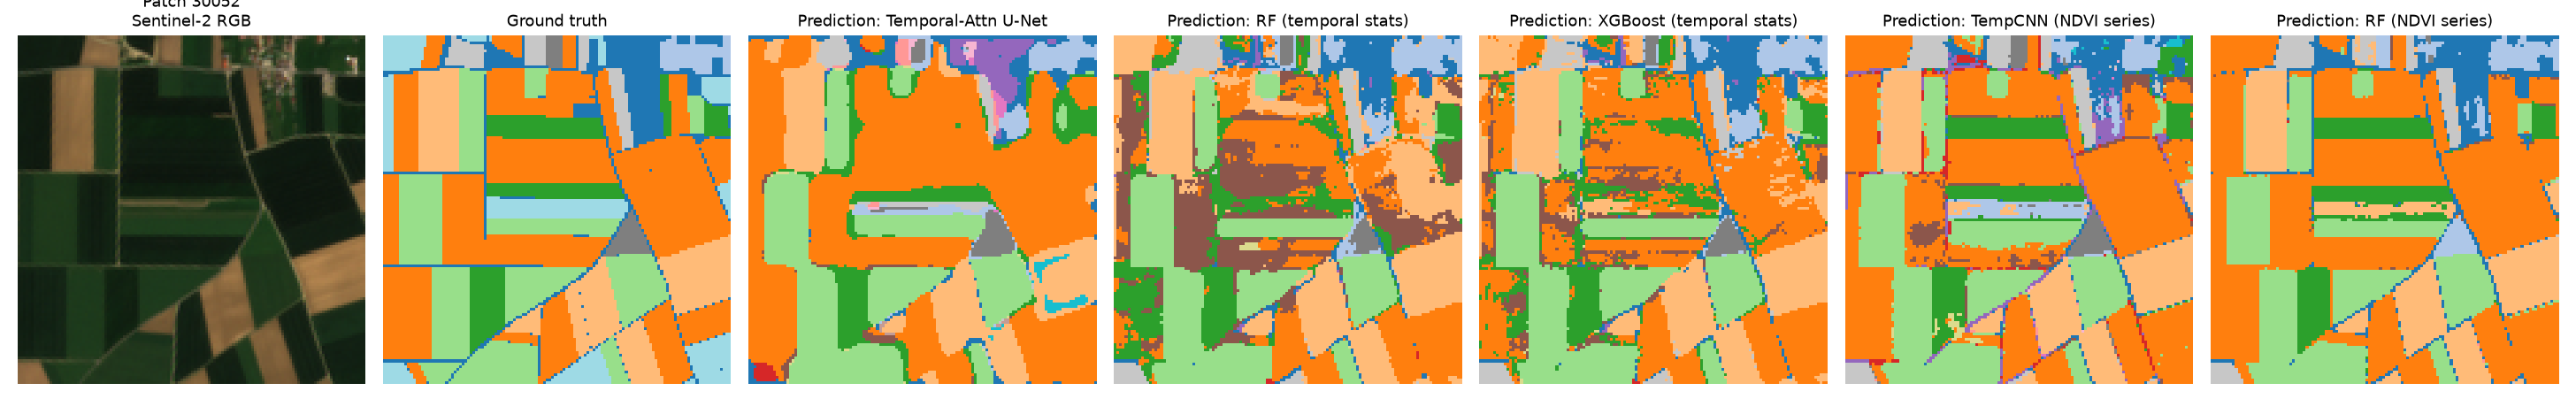
\includegraphics[width=\textwidth]{prediction_panel_patch_30052.png}
\caption{Test patch 30052: Sentinel-2 RGB, ground truth, and predictions from
every evaluated model. The delivered model (rightmost) reproduces parcel
geometry most closely.}
\label{fig:panel}
\end{figure}

The delivered model reproduces parcel geometry closely, with boundaries and
class assignments largely matching ground truth. Residual error concentrates at
parcel edges (mixed pixels) and as light within-parcel speckle --- expected,
since each pixel is classified independently with no spatial smoothing. For
contrast, the temporal-statistics models show heavy within-parcel noise and
systematic class confusion across whole fields, and the U-Net produces spatially
smooth output that is often confidently assigned to the wrong class.

%==============================================================================
\section{Conclusion and Next Steps}\label{sec:conclusion}
%==============================================================================

A Random Forest on the ordered NDVI time series classifies crop types at
\textbf{0.861 accuracy / 0.370 macro-F1 (0.475 over classes actually present)}
on a spatially disjoint, leakage-free split, reproducible in under three minutes
on a CPU. It beat a gradient-boosted variant, a 1D CNN on identical features,
and a converged Temporal-Attention U-Net on raw bands. The evidence supports a
specific, transferable conclusion: \textbf{for crop-type classification on small
satellite time-series datasets, preserving phenological timing in the feature
representation mattered about three times more than model capacity} --- and
model capacity actively hurt once the independent-sample count was this low.

Recommended next steps, in priority order:

\begin{enumerate}[leftmargin=*]
  \item \textbf{Combine ordering with the full spectrum} --- ordered series of
        all 10 bands, or ordered NDVI concatenated with Track~A statistics. The
        most promising cheap experiment, and it would disentangle ``ordering''
        from ``NDVI-only,'' which the current comparison confounds.
  \item \textbf{Make the representation calendar-robust} by resampling onto a
        fixed day-of-year grid (e.g.\ 24 fortnightly composites), removing the
        dependence noted above and enabling transfer to other tiles and years.
  \item \textbf{Run all five folds} to replace single-split point estimates with
        means and variances, which the rare-class metrics badly need.
  \item \textbf{Parcel-level majority voting} using the polygons already in
        \file{metadata.geojson} --- cheap post-processing that should remove the
        residual within-parcel speckle.
  \item \textbf{Explicit cloud handling} --- drop or interpolate the dates
        flagged in Section~\ref{sec:eda}, which corrupt individual features
        outright in this representation.
  \item \textbf{Evaluate on full PASTIS} ($\sim$2{,}433 patches) for
        statistically meaningful rare-class metrics, or group the rarest classes
        under a shared ``other'' label if data remains this scarce.
\end{enumerate}

%==============================================================================
\begin{thebibliography}{9}

\bibitem{garnot2021}
V.~S.~F. Garnot et al.,
\emph{Panoptic Segmentation of Satellite Image Time Series with Convolutional
Temporal Attention Networks}, ICCV 2021. (PASTIS dataset / U-TAE architecture.)
\url{https://github.com/VSainteuf/pastis-benchmark}

\bibitem{pelletier2019}
C.~Pelletier, G.~I. Webb, F.~Petitjean,
\emph{Temporal Convolutional Neural Network for the Classification of Satellite
Image Time Series}, Remote Sensing, 2019. (TempCNN, the Track~D architecture
family.)

\bibitem{rouse1974}
J.~W. Rouse et al.,
\emph{Monitoring Vegetation Systems in the Great Plains with ERTS}, NASA, 1974.
(NDVI.)

\bibitem{libs}
scikit-learn, XGBoost, PyTorch, GeoPandas and Rasterio --- see
\file{requirements.txt} for pinned versions.

\end{thebibliography}

\end{document}
